\documentclass[uplatex]{jsarticle}
\usepackage[dvipdfmx]{graphicx}
\usepackage{amsmath,amssymb}

\title{hoge}
\author{hoge}
\date{hoge}

\begin{document}
\maketitle

\section{hoge}

エネルギー$E$と質量$m$は
\begin{align}
    E = mc^2
\end{align}
で関係づけられる。

林檎を図\ref{apple}に示す。

\begin{figure}
    \centering
    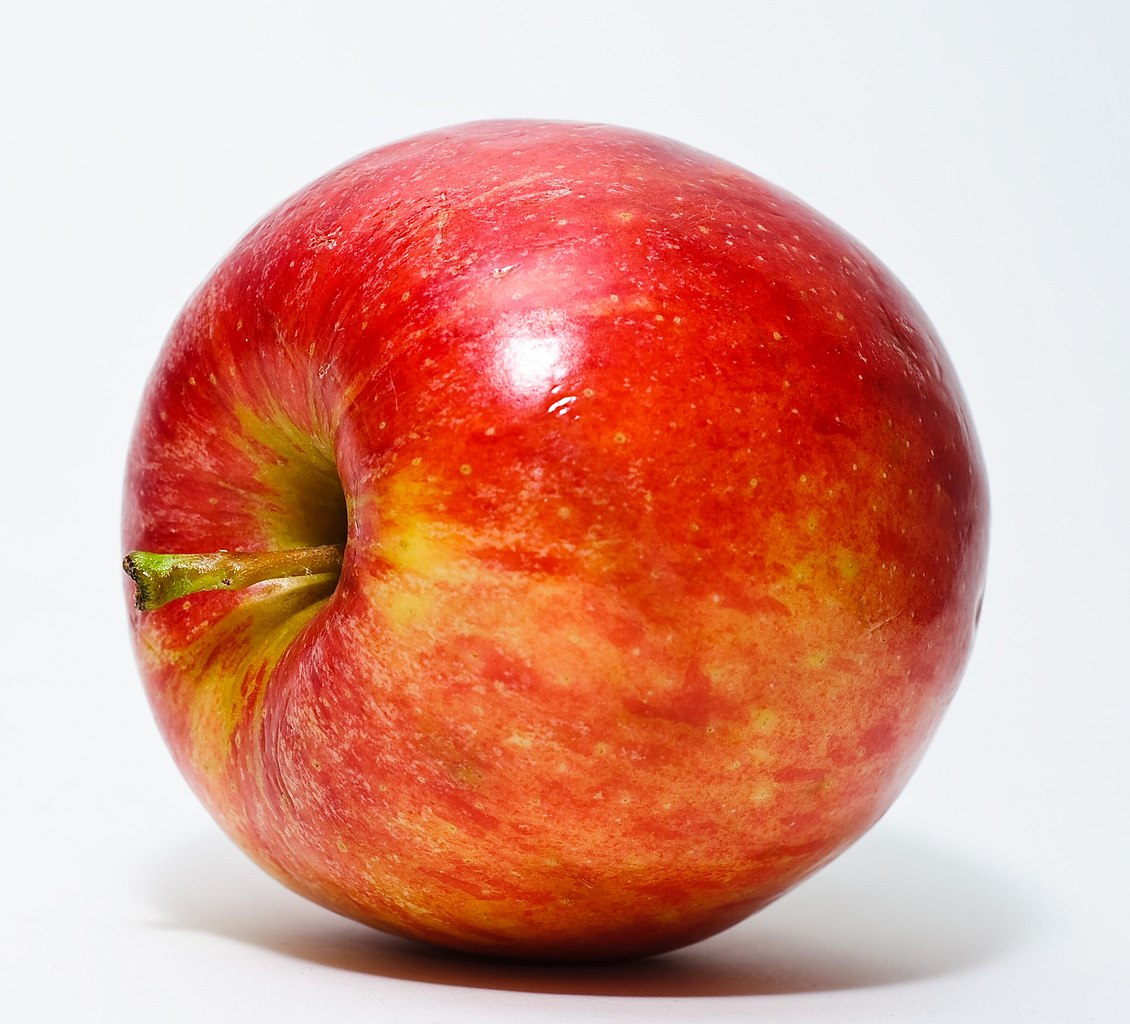
\includegraphics[width=10cm]{apple.jpg}
    \caption{林檎の図}
    \label{apple}
\end{figure}

\end{document}
